% !TEX root = ../thesis.tex

\chapter{Results and Discussion}\label{ch:results_discussion}

Vyhodnocovacia časť je kľúčovou časťou záverečnej práce. Tato časť obsahuje vyhodnotenie navrhnutého (vytvoreného) riešenia. Uprednostňované je objektívne vyhodnotenie výsledkov práce, ktoré sa opiera o meranie a štatistické metódy, prípadne matematické dôkazy. V prípade nameraných hodnôt musí autor opísať metódu merania, priebeh merania, výsledky a interpretáciu výsledkov v kontexte riešeného problému a stanovených cieľov. Na základe vyhodnotenia riešenia autor opíše prínosy svojej práce. Vyhodnocovacia časť tvorí zvyčajne ¼ jadra práce.

\section{Overview of Conducted Experiments}

This chapter presents the quantitative and qualitative results of the conducted experiments. The experiments were treated not as an independent sequence of model runs, but as a set of controlled experimental groups. Each group was designed to assess the impact of a single methodological component, such as input data representation, label representation, loss function, sampling strategy, or model architecture. This structure allows us to distinguish general trends from the specific results of individual configurations. A detailed description of all configurations will not be provided due to their high variability; they follow directly from the methodology described above and adhere to a defined evaluation protocol.

Experiments were conducted separately for the datasets on Maya structures and Slovak terraces, as these two study areas differ in object morphology, terrain context, and annotation characteristics. The Maya dataset focuses primarily on compact archaeological structures, whereas the Slovak dataset contains linear objects similar to terraces. Therefore, the results are presented separately for both areas and only then compared at the level of methodological trends. A complete description of the characteristics of the available data is provided in Chapter 4.

Only experiments conducted on the latest consistent version of the workflow will be considered to ensure the objectivity of the subsequent comparison and to minimize the impact of possible methodological drift from minor changes. This will ensure a meaningful comparison of the tested components regardless of the input data domain.

\begin{table}[htbp]
\centering
\small
\setlength{\tabcolsep}{4pt}
\renewcommand{\arraystretch}{1.25}

\begin{tabularx}{\textwidth}{@{}p{3.8cm} p{1.8cm} X@{}}
\toprule
\textbf{Component} &
\textbf{Study area} &
\textbf{Compared variants} \\
\midrule

\multirow{2}{=}{Input Data Representation} &
Maya &
DEM, RGB, RGDEM, SPS \\

&
Slovakia &
DEM, ISO, ANISO \\
\midrule

\multirow{2}{=}{Label Representation} &
Maya &
Hard mask, soft masks with different radius \\

&
Slovakia &
Hard mask and soft mask variants \\
\midrule

\multirow{2}{=}{Loss function} &
Maya &
BCE + Dice, Tanimoto, Focal-based losses, DECB \\

&
Slovakia &
BCE + Dice and Tanimoto with complement \\
\midrule

\multirow{2}{=}{Sampling Strategy} &
Maya &
128 and 256 pixel tiles with corresponding strides \\

&
Slovakia &
128, 256, 512, and 1024 pixel tiles \\
\midrule

\multirow{2}{=}{Model Architecture} &
Maya &
DeepLab V3, DeepLab V3+, pretrained DeepLab V3+ \\

&
Slovakia &
DeepLab V3, DeepLab V3+, pretrained DeepLab V3+ \\

\bottomrule
\end{tabularx}

\caption{Overview of the experimental groups evaluated on the Maya structures and Slovak terrace datasets.}
\label{tab:experiments_overview}
\end{table}

Table ~\ref{tab:experiments_overview} provides an overview of the main experimental groups that will be analyzed in this section. The table intentionally lists only the main controlled variables and comparison options. A complete list of experiments, including the number of configurations, settings with the best results, and detailed observations, is provided in the appendix ~\ref{app:tab:experiments_summary}. As noted earlier, the control variables consist of identified approaches by various authors proposing specific methods; however, most of them lack broader validation beyond the specific domain and selected configuration. In this context, the main goal of improving the stability of the results is not to segment existing structures while preserving the correct geometry, but rather to ensure that no potential candidate objects are overlooked that might be of interest in an expert review.

\section{Reference and Best-Performing Configurations}
\subsection{Best-Performing Configuration for Maya Structures}

For the available Maya data, the following configuration yielded the most promising results:
\begin{itemize}
    \item Model - DeepLab V3+ (IMAGENET Pretrained ResNet-101 backbone)
    \item Input representation: SPS (radius = 10m, n\_dir = 16, noise\_sup=0, z-score normalization)
    \item Labels: Soft mask (radius = 2m)
    \item Loss Function: Tanimoto with complement loss
    \item Tile Size: 128x128px (stride = 32px)
\end{itemize}
Existing research indicates that pretrained weights provide a significant advantage during training, accelerating convergence and typically improving metrics. However, to compare the impact of pretrained weights, we will compare these results with the same configuration but using the older DeepLab V3 model without pretrained weights. The reason for comparing specifically with the older model lies in the minimal difference in performance between the DeepLab V3 and V3+ models without pre-trained weights, as the difference in results according to evaluation metrics is less than 1 percent, and visual validation did not reveal any significant differences.

Due to the lack of objectivity of pixel-based metrics in the context of the current task, an object-based analysis was also conducted to identify the actual results of the inference. However, pixel metrics remain a necessary indicator during training; they are specifically addressed in Table~\ref{tab:maya_v3_v3+_metrics}. Some metrics do not reflect useful information, as described in Section~\#, so only those that truly reflect useful training information were retained for comparison. It is immediately apparent that the DeepLab V3+ model is the clear leader across all pixel-based evaluation metrics. At the same time, the object-based evaluation, showed in Table~\ref{tab:maya_v3_v3+_object_metrics}, also demonstrates the superiority of the more modern model. Overall, both models handle segmentation relatively well, segmenting between 43\% and 61\% of the available 4084 objects regardless of size. Furthermore, the models make mistakes in the same locations, where isolated small objects are situated on blurred terrain, making their detection more difficult, or conversely, where natural terrain mimics a morphology very similar to man-made structures. A detailed overview of each scenario is shown in Figure~\ref{fig:maya_tp_fp_fn_comparison}. The only difference between the newer model and its predecessor is the lower number of false-positive predictions—the model detects even fragments of potential buildings, so fewer potential candidates would be missed during manual analysis.

\begin{table}[!ht]
    \centering
    \caption{DeepLab V3 \& DeepLab V3+ pixel-wise metrics comparion on Maya dataset}
    \begin{tabular}{|l|ll|}
    \hline
        \textbf{Metric / Model} & \textbf{DeepLab V3} & \textbf{DeepLab V3+} \\ \hline
        \textbf{Balanced Accuracy} & 0.68021 & 0.72479 \\ 
        \textbf{True Positive Rate} & 0.36169 & 0.45008 \\ 
        \textbf{Positive Predictive Value} & 0.43755 & 0.70669 \\ 
        \textbf{F1 Score} & 0.39602 & 0.54992 \\ 
        \textbf{IoU (Foreground)} & 0.24690 & 0.37924 \\ 
        \textbf{IoU (Average)} & 0.62196 & 0.68862 \\ 
        \textbf{Matthews Correlation Coefficient} & 0.39634 & 0.56307 \\ \hline
    \end{tabular}
    \label{tab:maya_v3_v3+_metrics}
\end{table}

\begin{table}[!ht]
    \centering
    \caption{DeepLab V3 \& DeepLab V3+ object-wise metrics comparion on Maya dataset}
    \begin{tabular}{|l|ll|}
    \hline
        \textbf{Metric / Model} & \textbf{DeepLab V3} & \textbf{DeepLab V3+} \\ \hline
        \textbf{Detected GT Object} & 1746 & 2253 \\ 
        \textbf{Average pixels hit-rate per object} & 93.6 & 90.27 \\ 
        \textbf{Predicted Objects} & 1792 & 2528 \\ 
        \textbf{TP Predictions} & 1642 & 2248 \\ 
        \textbf{FP Predictions} & 150 & 280 \\ \hline
    \end{tabular}
    \label{tab:maya_v3_v3+_object_metrics}
\end{table}

\begin{figure}[htbp]
    \centering
    \begin{subfigure}{0.49\textwidth}
        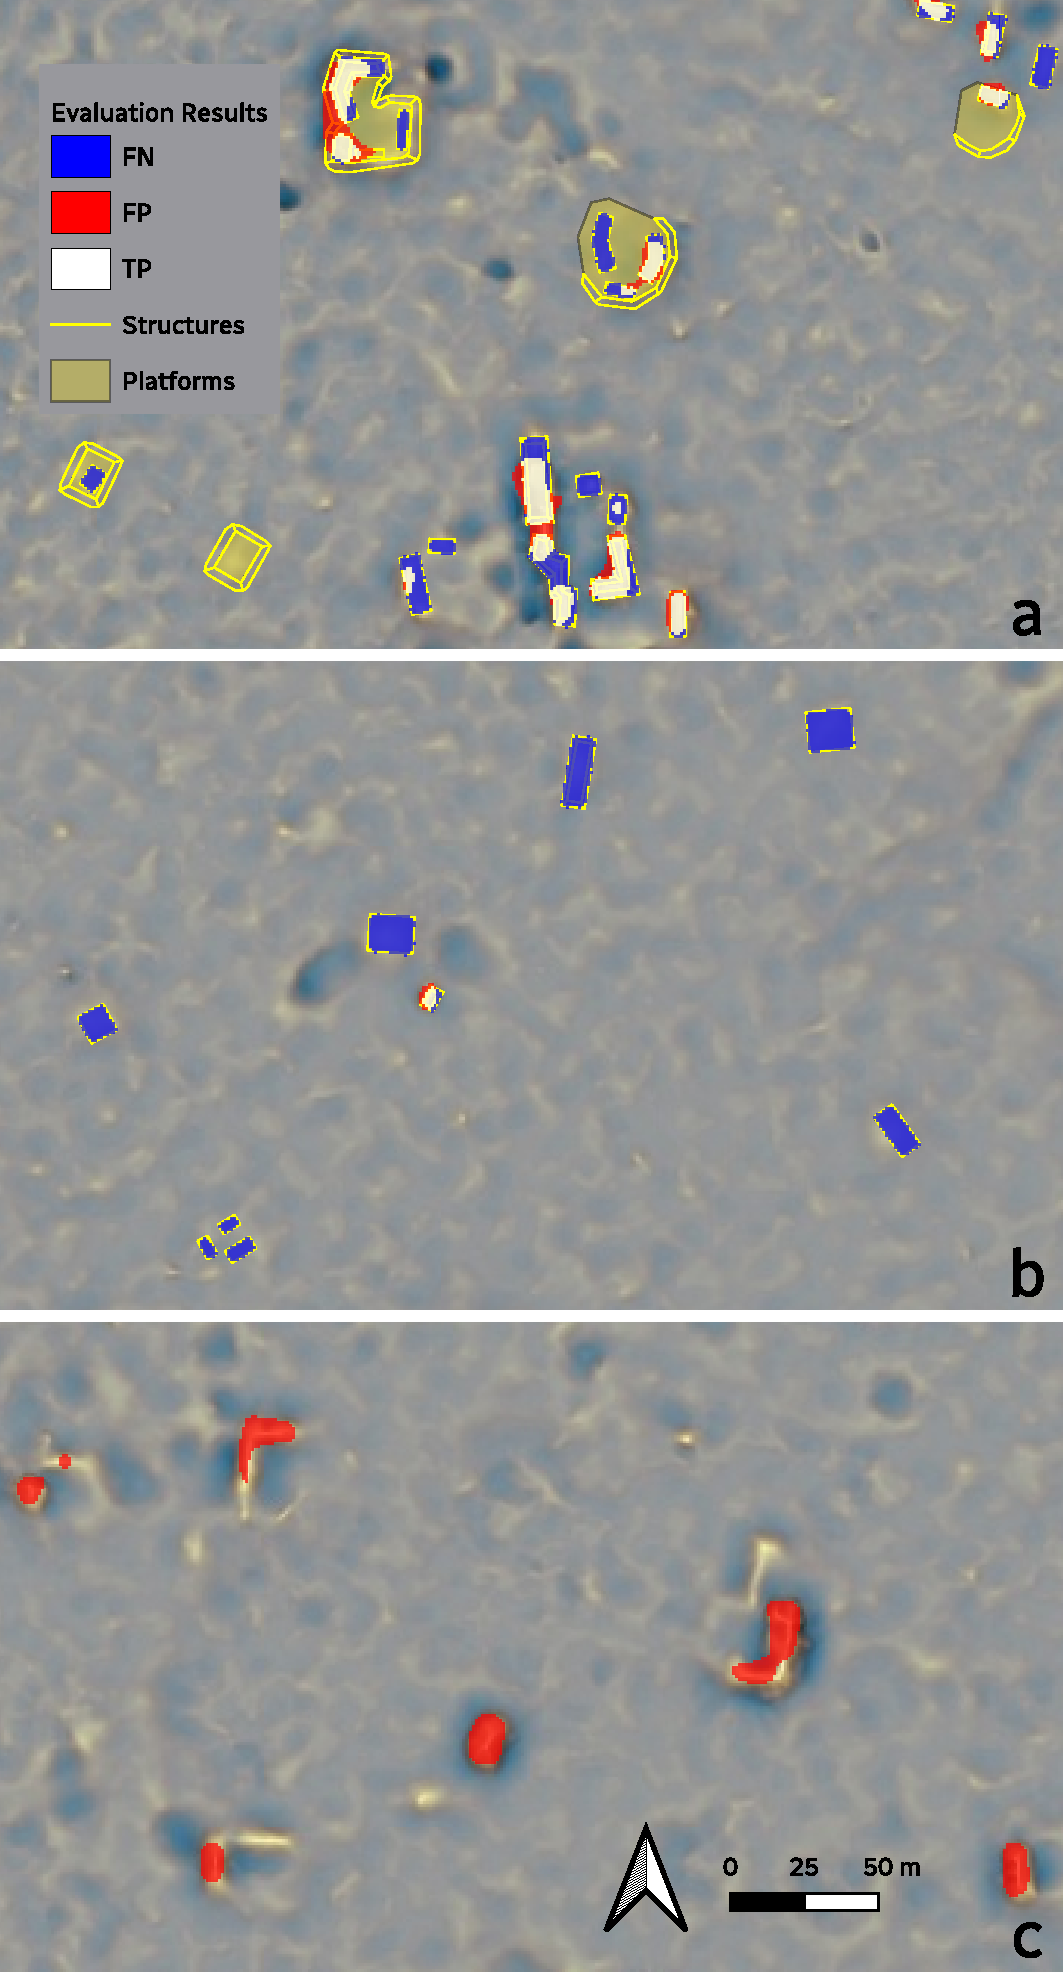
\includegraphics[width=\textwidth]{figures/maya_tp_fp_fn_sps_v3.pdf}
        \caption{DeepLab V3}
        \label{fig:maya_v3}
    \end{subfigure}
    \hfill
    \begin{subfigure}{0.49\textwidth}
        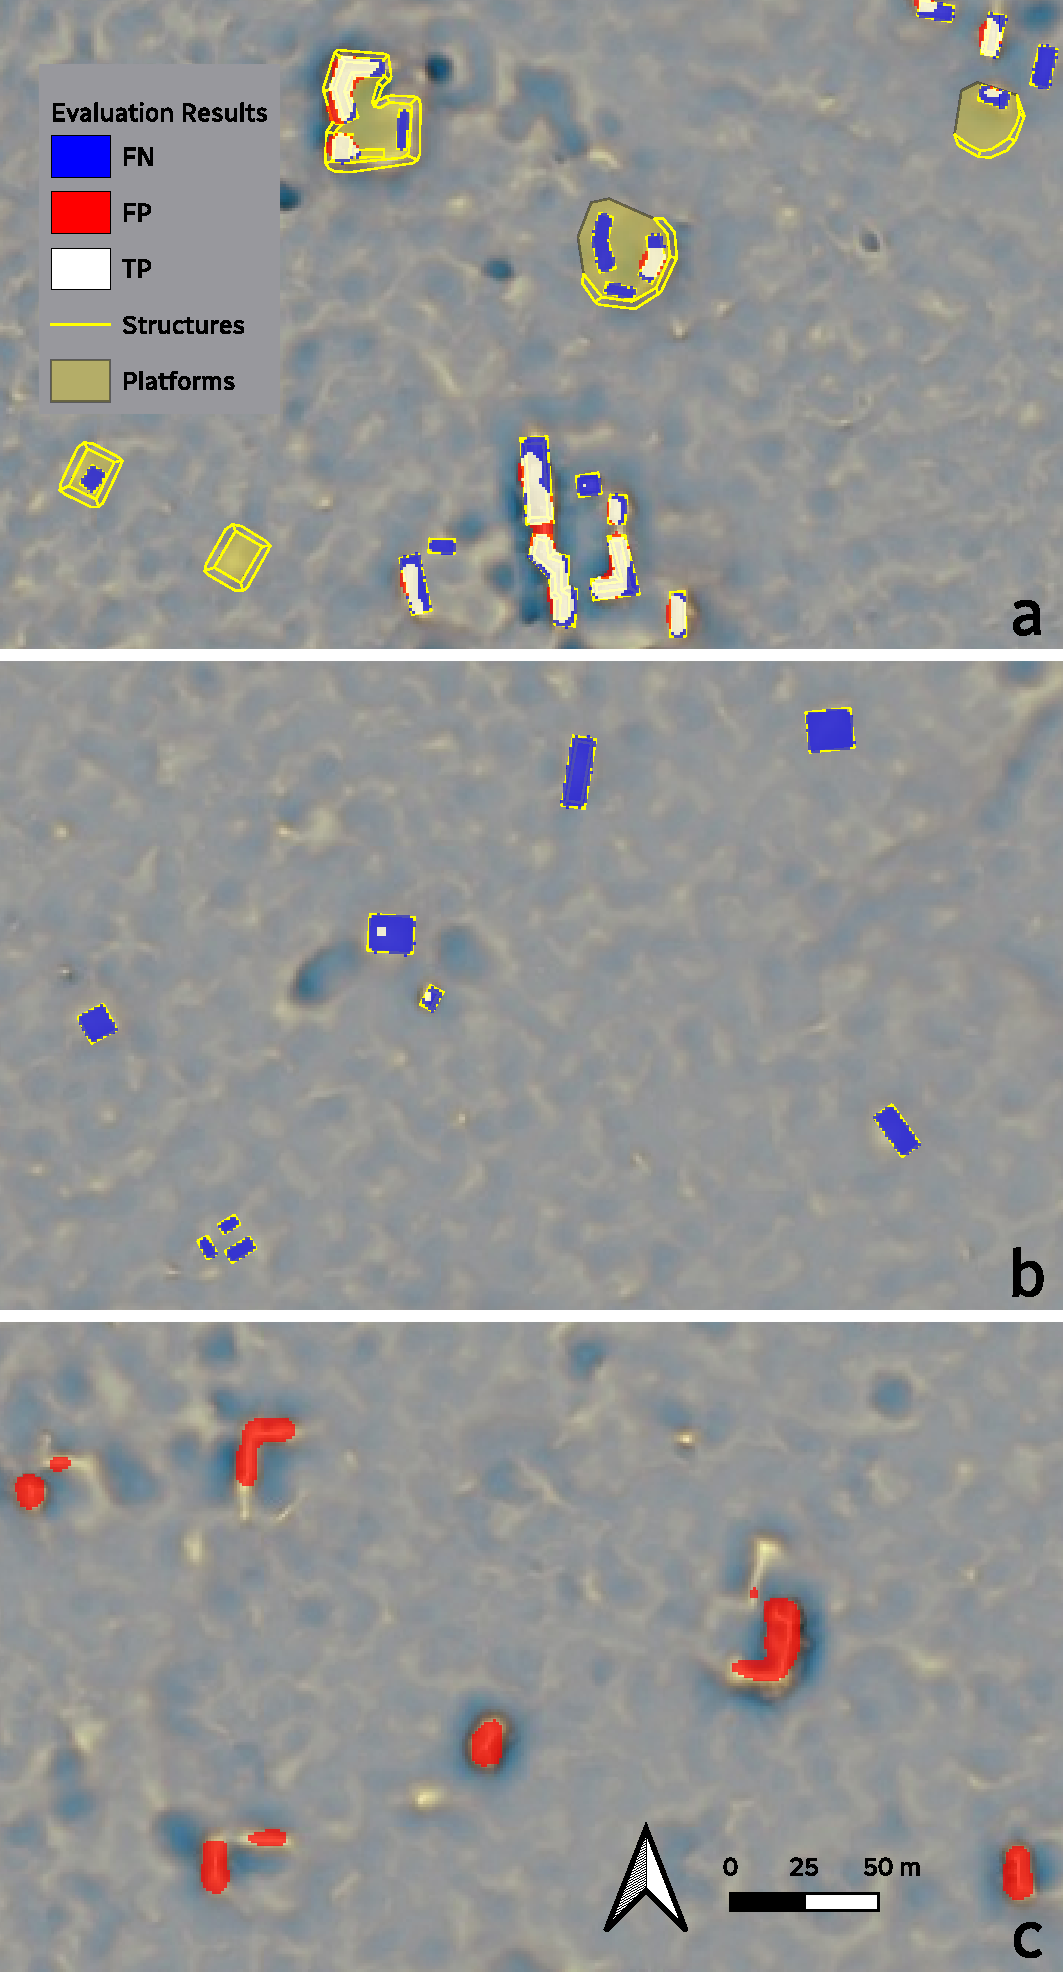
\includegraphics[width=\textwidth]{figures/maya_tp_fp_fn_sps_v3+.pdf}
        \caption{DeepLab V3+}
        \label{fig:maya_v3_plus}
    \end{subfigure}
    \caption{Comparison of the number of true positives, false positives, and false negatives for DeepLab V3 and DeepLab V3+ models on the Maya dataset.}
    \label{fig:maya_tp_fp_fn_comparison}
\end{figure}

\subsection{Best-Performing Configuration for Slovak Terraces}
\section{Ablation Study}
\subsection{Effect of Input Representation}
\subsection{Effect of Label Representation}
\subsection{Effect of Sampling Strategy}
\subsection{Effect of Loss Function}
\subsection{Effect of Tile Size of Inference Strategy}
\section{Error Analysis}
\section{Archaeological Usefulness of the Results}
\section{Limitations}
